\documentclass[conference]{IEEEtran}
\usepackage[utf8]{inputenc}
\usepackage[T1]{fontenc}
\usepackage{graphicx}
\usepackage{amsmath,amssymb}
\usepackage{booktabs}
\usepackage{hyperref}
\graphicspath{{../figs/}{photos/}}

% let floats pack densely so figures stay near their text
\renewcommand{\topfraction}{0.95}
\renewcommand{\bottomfraction}{0.95}
\renewcommand{\textfraction}{0.05}
\renewcommand{\floatpagefraction}{0.85}
\setcounter{topnumber}{4}
\setcounter{bottomnumber}{4}
\setcounter{totalnumber}{8}

\title{Antenna Measurements at Sub-THz Frequencies:\\
Communications Laboratory Report (Lab 2 \& 3), EE4730}

\author{\IEEEauthorblockN{Daniel Tyukov}
\IEEEauthorblockA{Student number 5714699 \\
Department of Microelectronics, TU Delft \\
d.a.tyukov@student.tudelft.nl \\
Measurement group G2}}

\begin{document}
\maketitle

\begin{abstract}
This report characterizes three antennas in the 140--220\,GHz band (WR-5.1): a 20\,dBi pyramidal horn, an open-ended waveguide probe, and a 30\,mm leaky-wave lens antenna. All measurements use a Keysight N5224B network analyzer with VDI frequency extenders, calibrated at the waveguide flanges. Time gating removes multipath ripple from every S-parameter trace. The extracted horn gain is 17.6--20.5\,dBi across the band, about 1.4\,dB below the datasheet values; the difference is consistent with the horn phase centres lying behind the aperture planes. The horn directivity from a far-field scan is 20.2\,dBi at 165\,GHz, and the probe gain is 5.9--7.5\,dBi. A focal-plane scan of the lens antenna reproduces the Airy pattern of a uniform 30\,mm aperture, with first sidelobes at $-17.5$\,dB and a directivity of 32--36\,dBi (aperture efficiency $\approx$\,0.8). The lens-to-lens link at $R=11.5$\,cm couples $-3.6$\,dB, while the Friis equation predicts an unphysical $+8.8$\,dB: the link operates deep in the radiative near field, where a quasi-optical model ($-1.9$\,dB) describes the measurement well. The remaining 1.7\,dB corresponds to about 0.9\,dB of reflection and ohmic loss per antenna, which puts the lens gain near 32.5\,dBi at 165\,GHz.
\end{abstract}

\section{Introduction and measurement setup}
The goal of this laboratory is to evaluate the coupling between antennas at sub-THz frequencies and to extract radiation patterns, directivity and gain from two-port S-parameter measurements \cite{lab1,lab2}. The setup is a Keysight N5224B PNA driving two VDI WR-5.1 frequency extenders (140--220\,GHz, 801 points, 100\,MHz spacing). A SOLT calibration with the WR-5.1 waveguide kit places the reference planes at the antenna flanges, so the measured $S_{21}$ is the antenna-to-antenna transfer function. Fig.~\ref{fig:setup} shows the transmit and receive modules and the calibration kit.

Four configurations were measured:
\begin{enumerate}
  \item Horn to horn at $R=10.5$\,cm: gain extraction by the two-antenna method.
  \item Horn to probe at $R=17.6$\,cm: the probe scans 41 positions along $x$ (5\,mm steps, H-plane) to map the horn far-field pattern.
  \item Lens to probe: the probe scans the focal plane of the lens system ($F=11.5$\,cm) in 1\,mm steps.
  \item Lens to lens at $R=11.5$\,cm: coupling of the quasi-optical link.
\end{enumerate}
The horn is an Eravant SAR-2013-05-S2 WR-05 pyramidal horn with a nominal gain of 20\,dBi \cite{eravant}. The lens antenna is a leaky-wave waveguide feed under a 30\,mm plastic elliptical lens \cite{bosma}. All processing was done in MATLAB; the scripts and data are archived with this report.

\begin{figure}[!t]
\centering
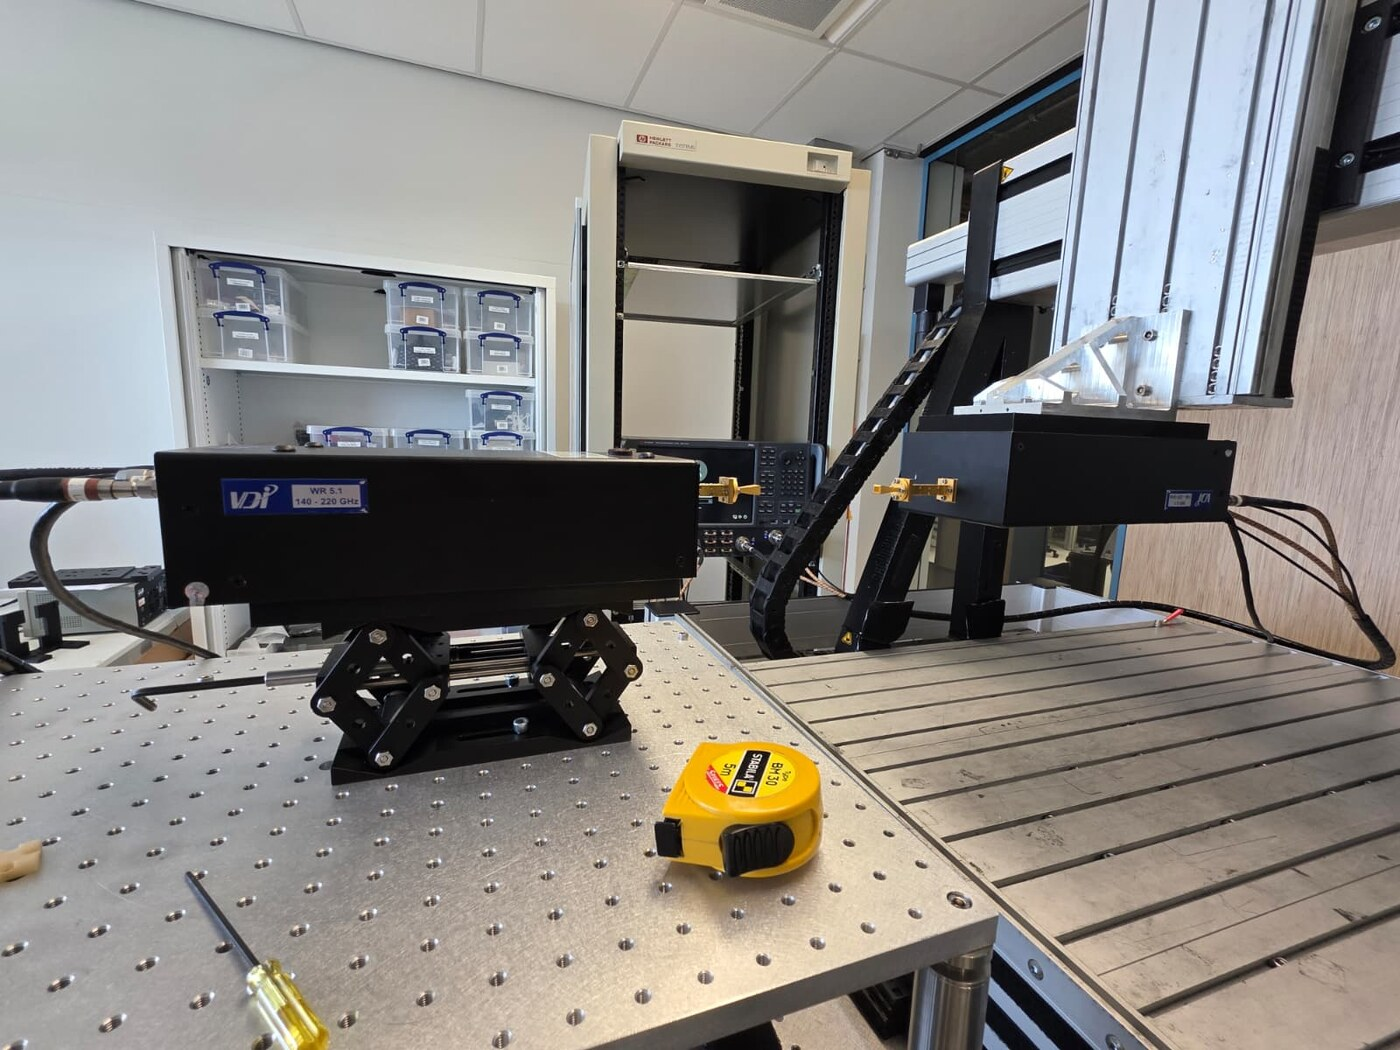
\includegraphics[width=0.49\columnwidth]{tx_rx_modules_facing_side_angle.jpg}\hfill
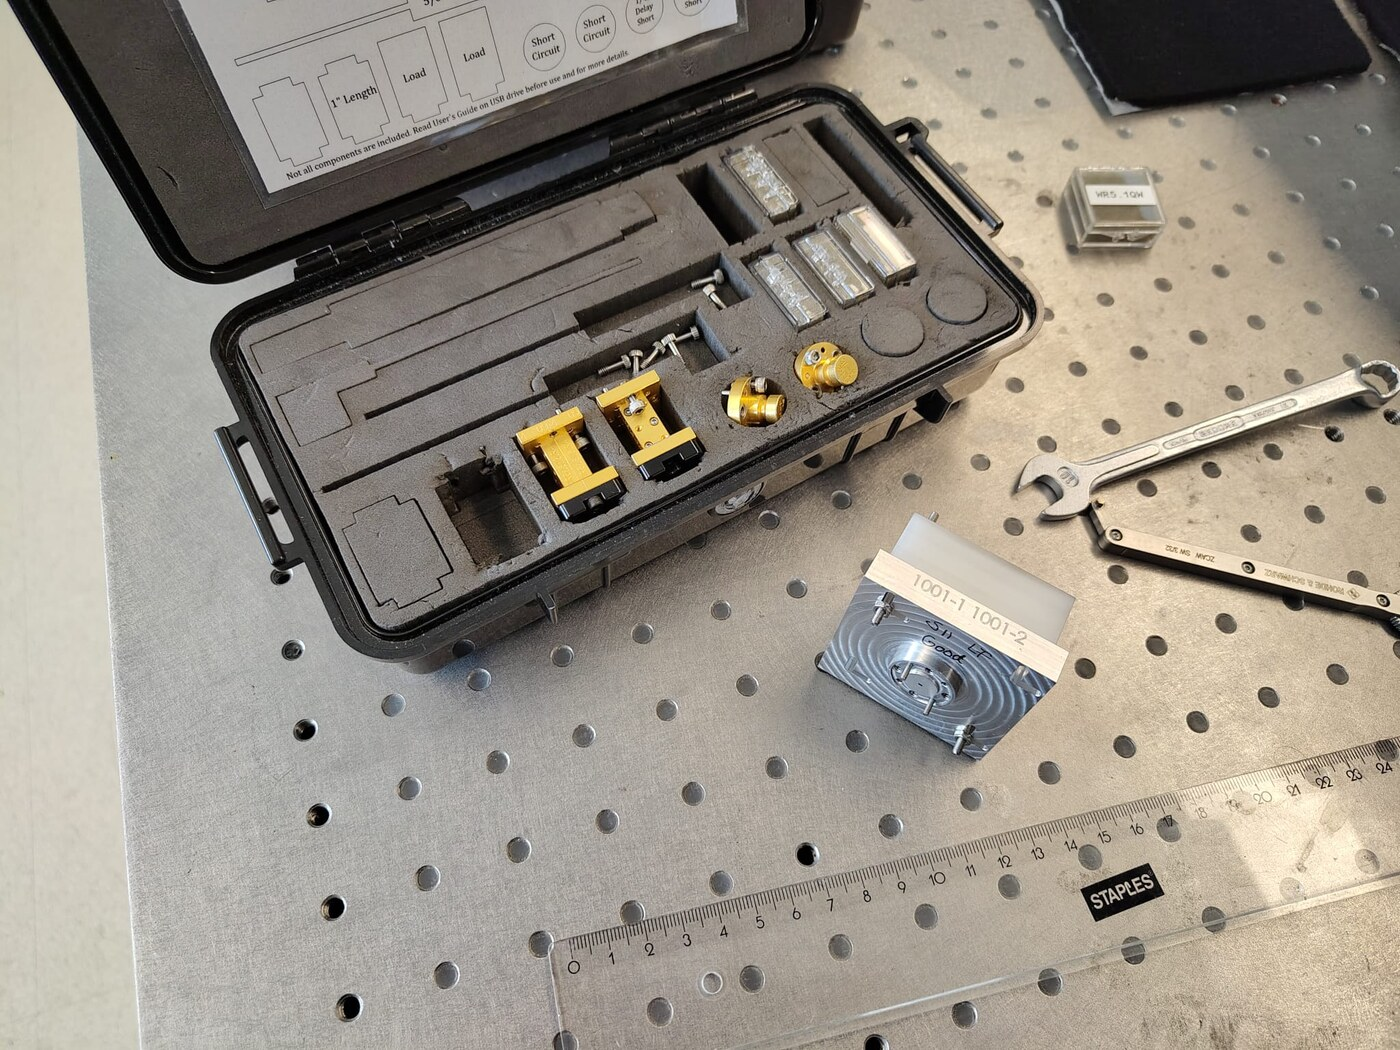
\includegraphics[width=0.49\columnwidth]{waveguide_calkit_open_with_ruler.jpg}
\caption{Left: VDI extender modules with the antennas facing each other. Right: WR-5.1 SOLT calibration kit.}
\label{fig:setup}
\end{figure}

\section{Time gating}
The lab bench is full of metal: extender housings, posts, the scanner itself. Reflections between these surfaces interfere with the direct path and produce ripple in $S_{21}(f)$. Because the sweep covers 80\,GHz in 100\,MHz steps, the inverse FFT of each trace gives the band-limited impulse response with 12.5\,ps resolution over an alias-free span of 10\,ns. The direct pulse and the multipath echoes separate cleanly in time, so a gate around the direct pulse removes the echoes; transforming back to the frequency domain gives the gated spectrum.

Fig.~\ref{fig:td}(a) shows the impulse responses of the two static links. The horn-to-horn pulse arrives at 0.56\,ns, which is $R/c = 0.35$\,ns plus the propagation through the two horns. The lens-to-lens response shows echo clusters at intervals of $2R/c \approx 0.77$\,ns after the main pulse: these are multiple round trips between the two lens apertures. The gate is a Tukey window of $\pm$0.25\,ns half-width centred on the direct pulse. In the scanned measurement the gate centre follows the geometric delay $r'(x)/c$, since the slant range grows by up to 90\,ps at the scan edges. Fig.~\ref{fig:gates} shows the raw and gated spectra: the ripple, $\pm$1.5\,dB peak-to-peak in the lens link, collapses onto a smooth curve. Gating distorts roughly the first and last 1.5\,GHz of the band (a gate of length $T$ smears spectral features by $1/T \approx 2$\,GHz), so derived quantities are only evaluated between 143.5 and 216.5\,GHz. A narrow interference spur near 211\,GHz survives gating in the low-level scan traces; the affected bands are masked in the directivity and probe-gain curves.

\begin{figure*}[!t]
\centering
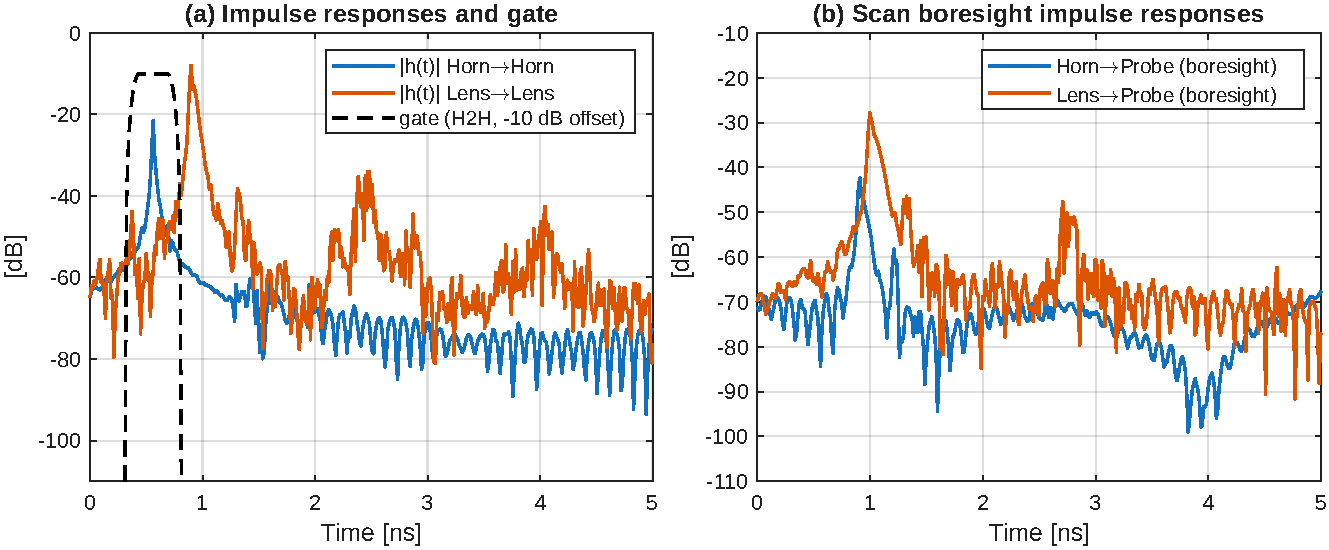
\includegraphics[width=0.85\textwidth]{fig_timedomain.pdf}
\caption{(a) Impulse responses of the horn-to-horn and lens-to-lens links with the time gate. (b) Boresight impulse responses of the two scanned measurements.}
\label{fig:td}
\end{figure*}

\begin{figure*}[!t]
\centering
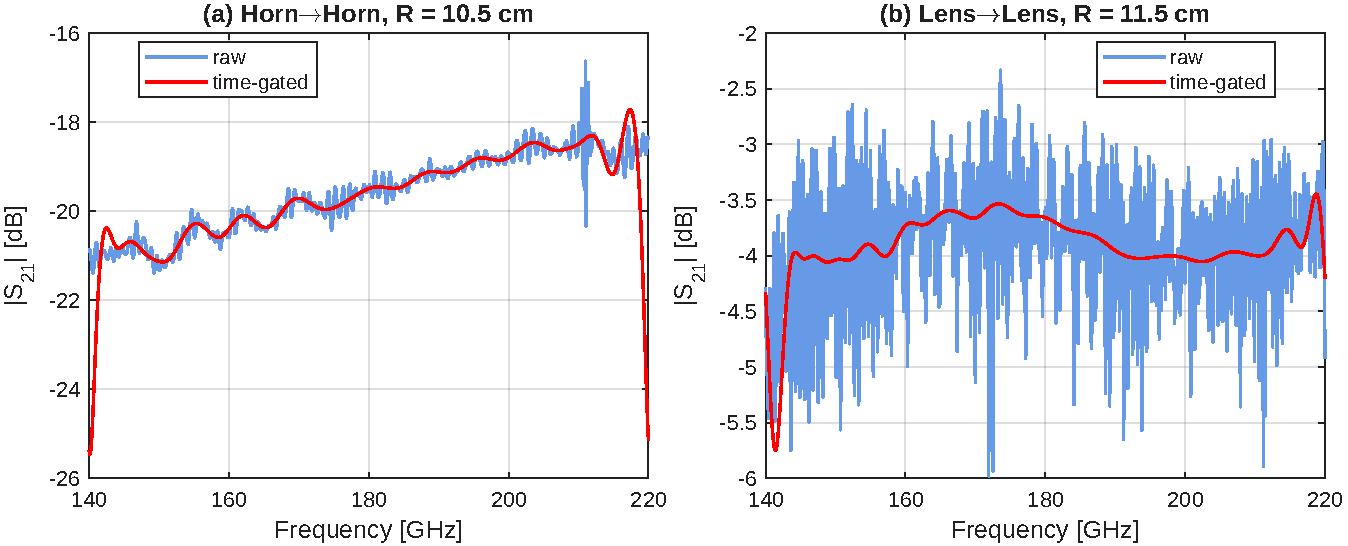
\includegraphics[width=0.85\textwidth]{fig_gating_s21.pdf}
\caption{Effect of time gating on the transmission of the two static links.}
\label{fig:gates}
\end{figure*}

\section{Horn antenna}
\subsection{Gain from the two-antenna method}
With two identical antennas in the far field, the Friis equation
\begin{equation}
\frac{P_{rx}}{P_{tx}} = G_{tx} G_{rx} \left(\frac{\lambda}{4\pi R}\right)^2
\label{eq:friis}
\end{equation}
gives the gain of each antenna directly from the gated transmission:
\begin{equation}
G(f) = \tfrac{1}{2}\left[\,|S_{21}|_{\mathrm{dB}} - 20\log_{10}\!\frac{\lambda}{4\pi R}\,\right].
\end{equation}
The far-field condition holds: $2D^2/\lambda \approx 4$\,cm for the horn, well below $R=10.5$\,cm. Fig.~\ref{fig:horngain} shows the result: the gain rises from 17.6\,dBi at 144\,GHz to 20.5\,dBi at 216\,GHz, with the same slope as the datasheet curve but about 1.4\,dB below it. The most likely cause is the distance definition. $R=10.5$\,cm was measured between the apertures, but the phase centre of a pyramidal horn sits behind the aperture, inside the flare. Placing the phase centres roughly 2\,cm behind each aperture makes the effective distance 14.5\,cm and raises the extracted gain by $10\log_{10}(14.5/10.5)=1.4$\,dB, which closes the gap. Residual misalignment also reduces the measured value but cannot raise it, so the extracted curve is a lower bound.

\begin{figure}[!t]
\centering
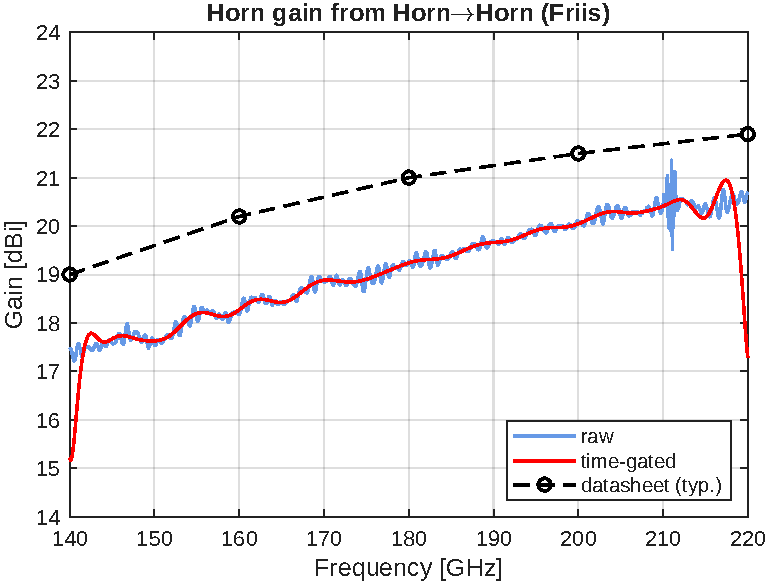
\includegraphics[width=\columnwidth]{fig_horn_gain.pdf}
\caption{Horn gain from the two-antenna method, raw and time-gated, compared with the manufacturer's typical gain \cite{eravant}.}
\label{fig:horngain}
\end{figure}

\subsection{Radiation pattern and directivity}
The probe samples the horn field along a line at $R=17.6$\,cm. The planar cut maps to angle by $\tan\theta = x/R$, and the field is compensated for the spherical spreading and phase to the scan plane:
\begin{equation}
E^{\mathrm{far}}(\theta) \propto S_{21}(x)\,\frac{r'}{R}\,e^{jk(r'-R)},\qquad r'=\sqrt{R^2+x^2},
\end{equation}
with the probe treated as ideal (its open-waveguide pattern is broad and flat over the $\pm 30^\circ$ covered here). Fig.~\ref{fig:hornpat} shows the gated H-plane patterns at 150, 165 and 195\,GHz. The main lobe narrows with frequency as expected from a fixed aperture. The dashed curve is the Airy pattern of the ideal uniform circular aperture with the same directivity as the horn at 165\,GHz ($D_{\mathrm{eq}}=5.9$\,mm): the measured main lobe matches it down to about $-10$\,dB, but the horn shows no nulls and a smooth skirt near $-20$\,dB, the usual consequence of the tapered (cosine) H-plane aperture distribution of a pyramidal horn.

Assuming rotational symmetry of the pattern, the directivity follows from the single cut,
\begin{equation}
D = \frac{2\,|E|^2_{\max}}{\int_0^{\theta_{\max}} |E(\theta)|^2 \sin\theta\, d\theta},
\label{eq:dir}
\end{equation}
where both half-cuts are averaged. The integration stops at $\theta_{\max}=30^\circ$, which truncates some radiated power and biases the estimate up by a fraction of a dB. Fig.~\ref{fig:horndir} compares the result with the Friis gain: $D$ is 19--22\,dBi across the band and follows the $f^2$ trend of the equivalent ideal aperture. At 165\,GHz the directivity is 20.2\,dBi and the half-power beamwidth is $19.0^\circ$. The 1.5--1.8\,dB offset between directivity and Friis gain contains the phase-centre bias discussed above plus the ohmic loss of the horn, so the two curves are mutually consistent.

\begin{figure}[!t]
\centering
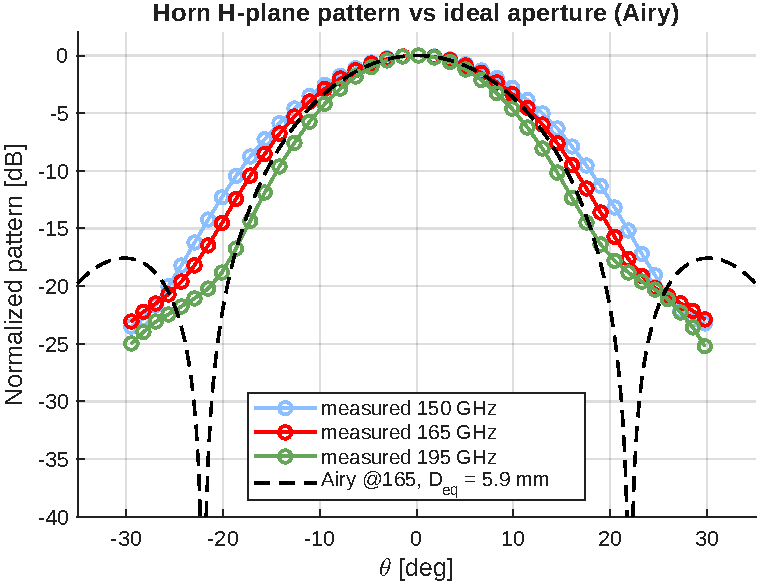
\includegraphics[width=\columnwidth]{fig_horn_pattern.pdf}
\caption{Measured H-plane patterns of the horn and the Airy pattern of the equal-directivity uniform aperture.}
\label{fig:hornpat}
\end{figure}

\begin{figure}[!t]
\centering
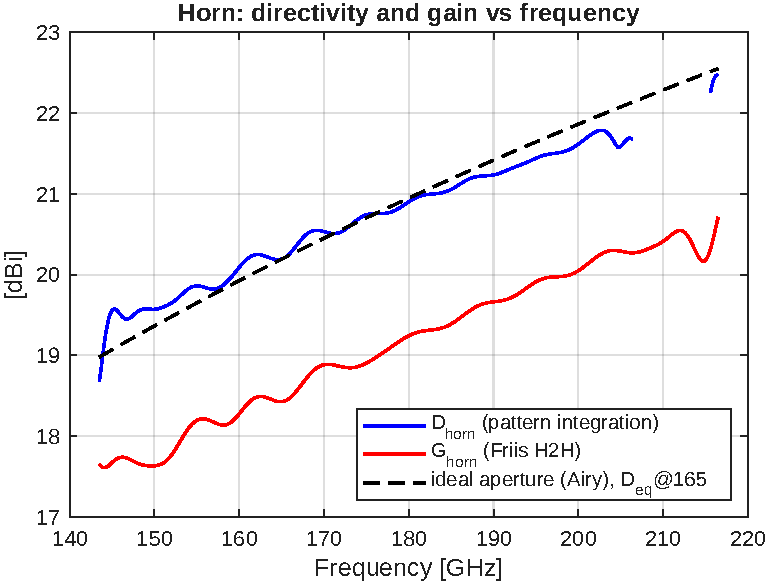
\includegraphics[width=\columnwidth]{fig_horn_dir_gain.pdf}
\caption{Horn directivity from pattern integration, Friis gain, and the directivity of the equal-directivity ideal aperture. The band around 211\,GHz is masked because of an interference spur.}
\label{fig:horndir}
\end{figure}

\subsection{Probe gain}
With the horn gain known, the boresight transmission of the horn-to-probe link gives the probe gain through \eqref{eq:friis}. Fig.~\ref{fig:probegain} shows 5.9\,dBi at 150\,GHz rising to 7.5\,dBi at 205\,GHz (6.3\,dBi at 165\,GHz), in the range expected for an open-ended rectangular waveguide. This estimate inherits the systematic uncertainty of the horn gain and of the distance definition.

\begin{figure}[!t]
\centering
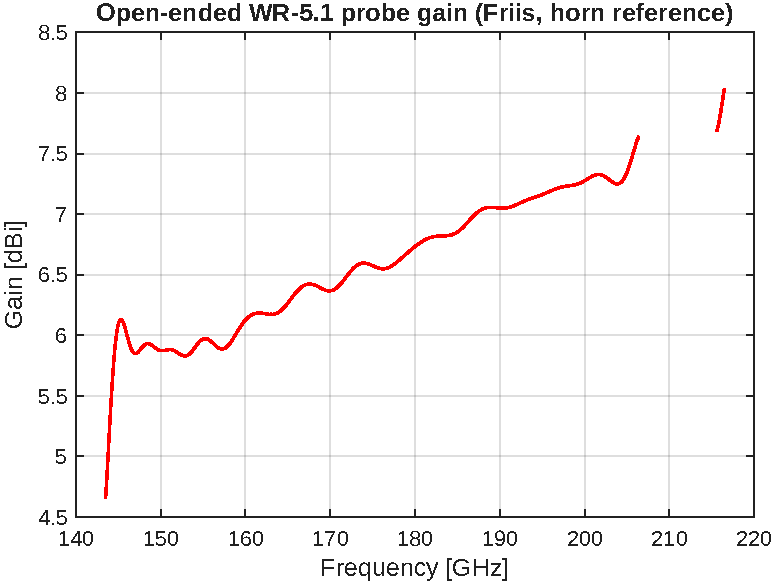
\includegraphics[width=\columnwidth]{fig_probe_gain.pdf}
\caption{Gain of the open-ended WR-5.1 waveguide probe.}
\label{fig:probegain}
\end{figure}

\section{Lens antenna}
\subsection{Focal-plane scan}
The lens measurement places the probe in the focal plane of the lens system at $F=11.5$\,cm. Fig.~\ref{fig:lensnf} shows the gated cut at 165\,GHz: an Airy-like spot with 7\,mm half-power width, first nulls near $\pm 10$\,mm and sidelobes at $-17.5$\,dB. The phase is flat within $\pm 10^\circ$ across the main lobe. Both observations identify the scan plane as the focal plane: a focusing aperture produces the spatial Fourier transform of its aperture field at the focus, so the focal field is the far-field pattern of the antenna read out at the scale $\sin\theta = x/F$ \cite{lab2}. The numbers agree quantitatively, since the Airy width $1.03\,\lambda F/D = 7.2$\,mm for $D=30$\,mm matches the measured spot.

\begin{figure*}[!t]
\centering
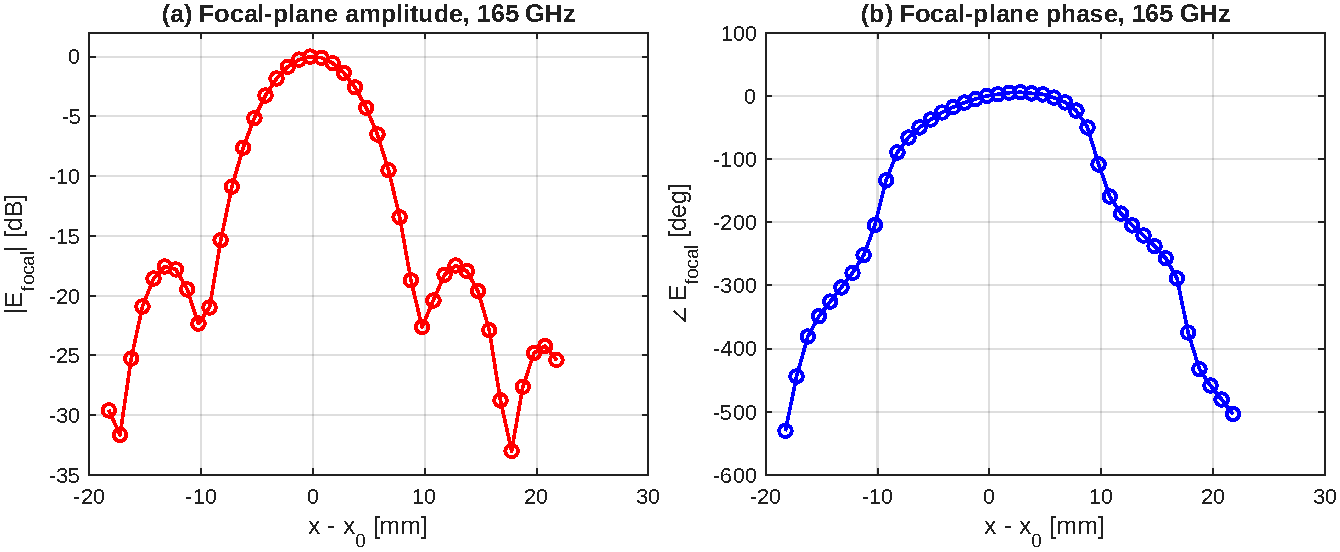
\includegraphics[width=0.85\textwidth]{fig_lens_nf.pdf}
\caption{Gated focal-plane cut of the lens antenna at 165\,GHz: (a) amplitude, (b) phase.}
\label{fig:lensnf}
\end{figure*}

\subsection{Pattern and directivity}
Fig.~\ref{fig:lenspat} shows the angular patterns at 150, 165 and 195\,GHz against the Airy pattern of a uniform 30\,mm aperture. The sidelobe level sits at the uniform-aperture value of $-17.5$\,dB at all three frequencies, so the lens illumination is close to uniform; this is the design goal of the leaky-wave feed \cite{bosma}. The main lobe is slightly wider than the ideal one (HPBW $4.0^\circ$ versus $3.6^\circ$ at 165\,GHz).

The directivity from \eqref{eq:dir} is shown in Fig.~\ref{fig:lensdir} together with the ideal-aperture limit $\pi^2 D_L^2/\lambda^2$. The measured curve runs 0.7--1.0\,dB below the limit across the whole band: 32.0\,dBi at 144\,GHz, 33.4\,dBi at 165\,GHz, 36.1\,dBi at 216\,GHz. The aperture efficiency is therefore $\approx 0.81$ at 165\,GHz, close to the published value of 0.85--0.88 for this antenna \cite{bosma}. The angular window of the scan is $\pm 11^\circ$, which truncates the integration in \eqref{eq:dir}; energy beyond the second sidelobe is neglected, so the true efficiency is marginally lower than quoted.

\begin{figure}[!t]
\centering
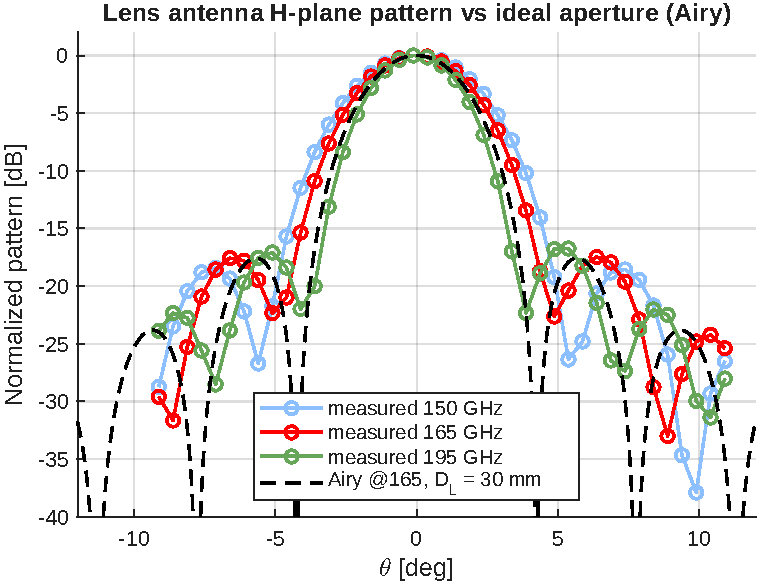
\includegraphics[width=\columnwidth]{fig_lens_pattern.pdf}
\caption{Lens antenna H-plane patterns from the focal-plane scan and the Airy pattern of the uniform 30\,mm aperture.}
\label{fig:lenspat}
\end{figure}

\begin{figure}[!t]
\centering
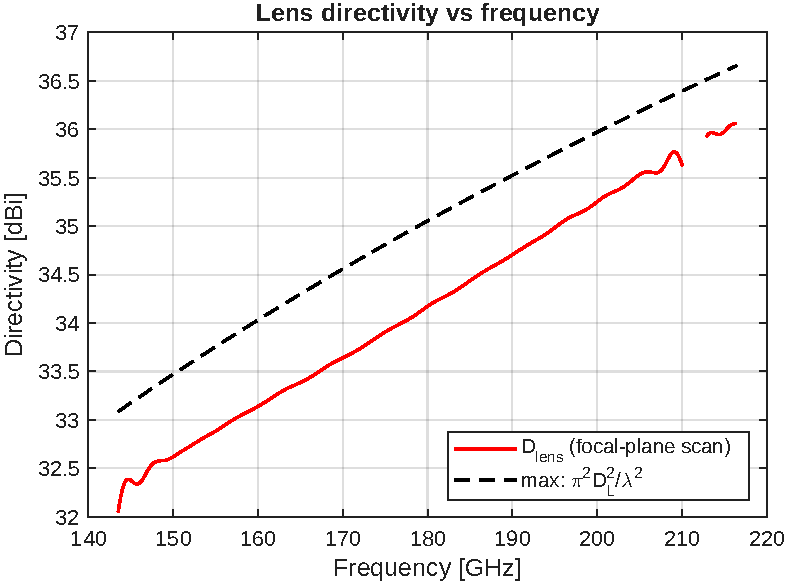
\includegraphics[width=\columnwidth]{fig_lens_dir.pdf}
\caption{Lens directivity against the ideal uniform-aperture limit.}
\label{fig:lensdir}
\end{figure}

\section{Coupling of the different setups}
Table~\ref{tab:summary} collects the link budgets at 165\,GHz. The horn link behaves classically: the measured $-20.4$\,dB equals the Friis prediction with the extracted gains, because the horns are in each other's far field.

The lens link does not. The two 30\,mm apertures sit 11.5\,cm apart, while the far-field distance of each is $2D_L^2/\lambda \approx 0.99$\,m at 165\,GHz. Inserting the measured directivities into \eqref{eq:friis} predicts $+8.8$\,dB, more power received than transmitted, which is impossible. Friis assumes spherical spreading over $R$, and inside the near field that assumption fails. The correct picture is quasi-optical: the collimated beam of one aperture barely spreads over 11.5\,cm and is intercepted almost entirely by the other aperture. The coupling between two uniform-phase apertures can be computed by propagating the aperture field with its plane-wave spectrum and evaluating the overlap integral with the receiving distribution,
\begin{equation}
\mathrm{Cou}(R) = \frac{\bigl|\iint E_1(R)\,E_2^{*}\, dS\bigr|^2}{\iint |E_1|^2 dS \,\iint |E_2|^2 dS}.
\end{equation}
Fig.~\ref{fig:coupling} shows this model next to the Friis lines and the two measured points. The quasi-optical curve stays within 2.5\,dB of full transmission until $R\approx 0.4$\,m and merges with Friis beyond the far-field distance. The measured lens-to-lens coupling of $-3.6$\,dB sits 1.7\,dB below the lossless model value of $-1.9$\,dB. Splitting the difference equally gives about 0.9\,dB of reflection plus ohmic loss per lens antenna, and a gain estimate of $33.4 - 0.9 \approx 32.5$\,dBi at 165\,GHz, consistent with the full-wave simulated gain of this antenna \cite{bosma}.

This comparison is the main lesson of the lab: at sub-THz frequencies, electrically large antennas put practical link distances inside the radiative near field, where a link can transfer almost all of its power. The Friis equation is then no longer a valid design tool, and quasi-optical coupling models take its place \cite{lab2}.

\begin{table}[!t]
\centering
\caption{Link summary at 165\,GHz (time-gated).}
\label{tab:summary}
\setlength{\tabcolsep}{4pt}\begin{tabular}{lccc}
\toprule
 & Horn$\to$Horn & Lens$\to$Lens & Horn$\to$Probe \\
\midrule
$R$ [cm] & 10.5 & 11.5 & 17.6 \\
$2D^2/\lambda$ [m] & 0.04 & 0.99 & 0.04 \\
Measured $|S_{21}|^2$ [dB] & $-20.4$ & $-3.6$ & $-37.0$ \\
Friis, extracted gains [dB] & $-20.4$ & $+8.8$ & $-37.0$ \\
QO model [dB] & -- & $-1.9$ & -- \\
\bottomrule
\end{tabular}
\par\smallskip
\footnotesize The horn and probe gains are extracted from the first and third links, so those Friis entries match by construction; applying the same procedure to the lens link fails because $R \ll 2D_L^2/\lambda$.
\end{table}

\begin{figure}[!t]
\centering
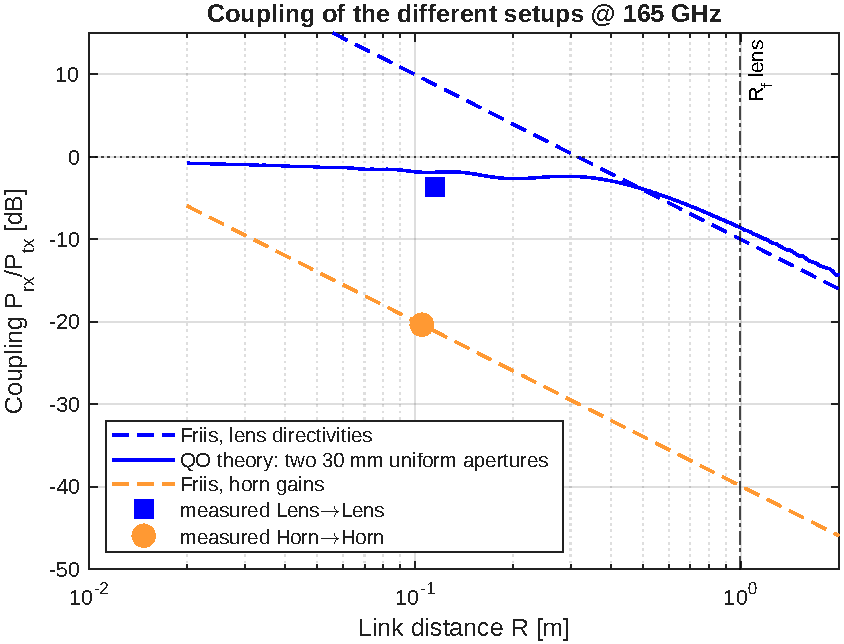
\includegraphics[width=\columnwidth]{fig_coupling.pdf}
\caption{Measured couplings at 165\,GHz against the Friis equation and the quasi-optical model for two 30\,mm uniform apertures. Fig.~\ref{fig:lensl2l} shows the corresponding bench setup.}
\label{fig:coupling}
\end{figure}

\begin{figure}[!t]
\centering
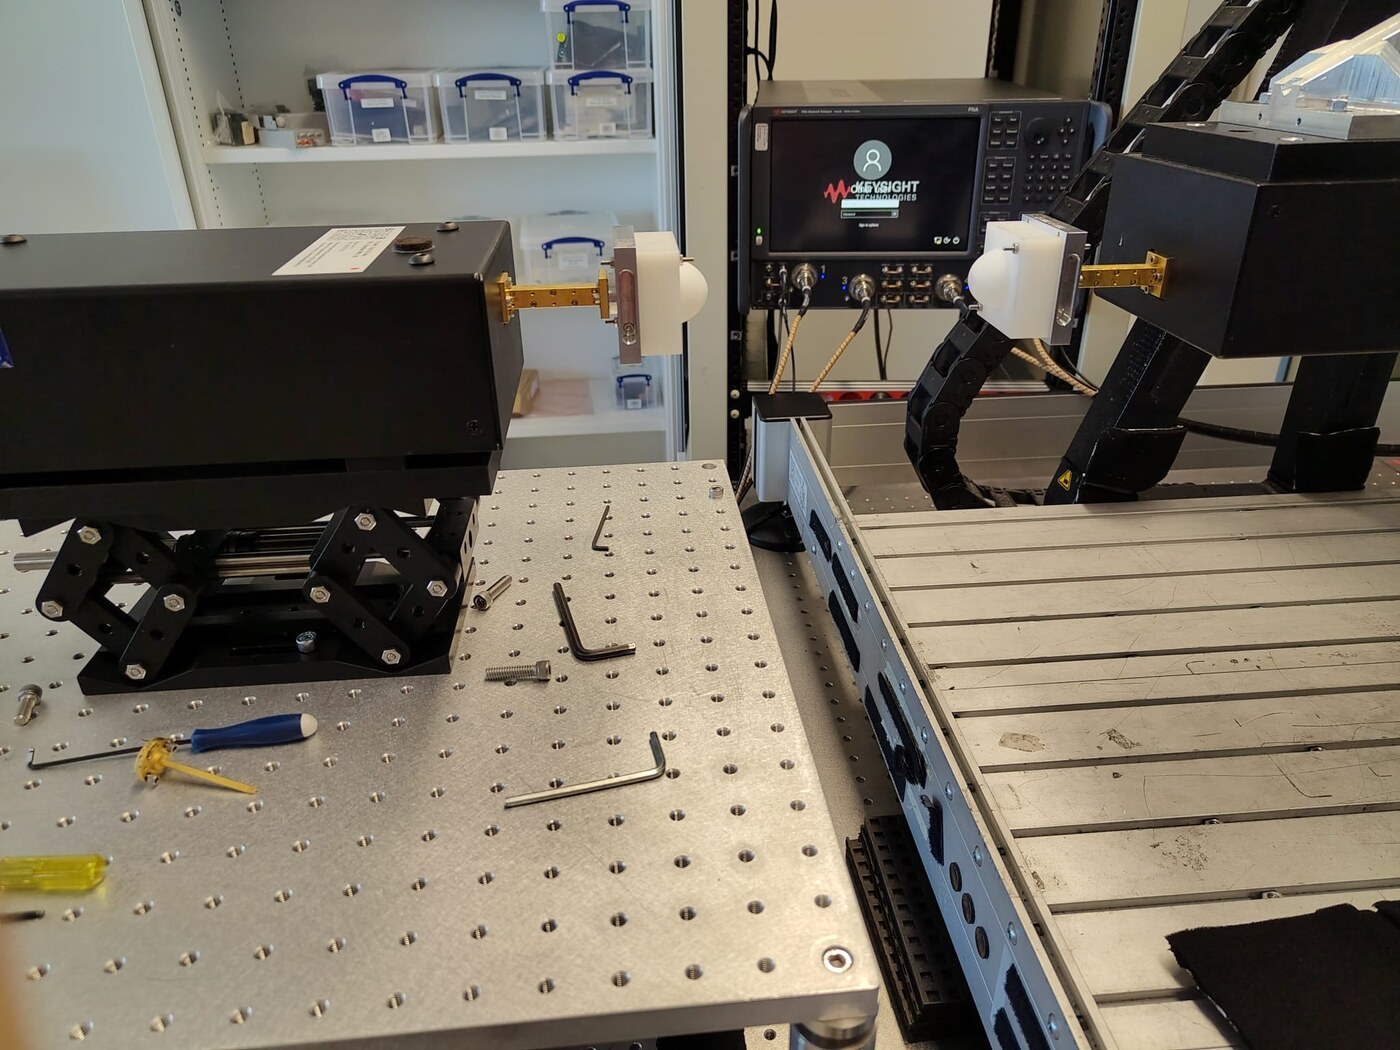
\includegraphics[width=0.8\columnwidth]{tx_rx_both_lens_antennas_facing.jpg}
\caption{The two lens antennas facing each other in the lens-to-lens configuration.}
\label{fig:lensl2l}
\end{figure}

\section{Conclusion}
Time gating turned heavily rippled raw spectra into clean transfer functions and made all further extraction possible; the gate parameters follow directly from the measured impulse responses. The horn measurements gave a gain of 17.6--20.5\,dBi and a directivity of 19--22\,dBi across 144--216\,GHz, both consistent with the datasheet once the phase-centre position is taken into account, and a probe gain of 5.9--7.5\,dBi. The focal-plane scan of the leaky-wave lens antenna reproduced the Airy distribution of a uniform 30\,mm aperture, with directivity 32--36\,dBi and aperture efficiency near 0.8. The coupling comparison showed the breakdown of the Friis equation in the radiative near field: the lens link at 11.5\,cm transfers $-3.6$\,dB of its power where Friis predicts an impossible $+8.8$\,dB, and a quasi-optical overlap model reproduces the measurement to within the antenna losses.

\begin{thebibliography}{9}
\bibitem{lab1} M. Alonso-delPino, ``EE4730 Project 2: Antenna measurements at sub-THz frequencies (Part 1),'' TU Delft, 2026.
\bibitem{lab2} M. Alonso-delPino, ``EE4730 Project 2: Antenna measurements at high frequencies. Far-field and near-field (Part 2),'' TU Delft, 2026.
\bibitem{eravant} Eravant, ``SAR-2013-05-S2: WR-05 pyramidal horn antenna, 20 dBi gain,'' datasheet.
\bibitem{bosma} S. Bosma, N. van Rooijen, M. Alonso-delPino, and N. Llombart, ``A wideband leaky-wave lens antenna with annular corrugations in the ground plane,'' \emph{IEEE Antennas Wireless Propag. Lett.}, 2022.
\bibitem{balanis} C. A. Balanis, \emph{Antenna Theory: Analysis and Design}, 4th ed. Wiley, 2016.
\end{thebibliography}

\end{document}
